\documentclass[journal,twocolumn]{IEEEtran}

\usepackage[utf8]{inputenc}
\usepackage{graphicx}
\usepackage{amssymb}
\usepackage{mathtools}
\usepackage{amsmath}
\providecommand{\pr}[1]{\ensuremath{\Pr\left(#1\right)}}
\providecommand{\cbrak}[1]{\ensuremath{\left\{#1\right\}}}

\title{Assignment 6}
\author{Gollapudi Sasank CS21BTECH11019}

\begin{document}
\maketitle
\section*{Question : }
In a factory which manufactures bolts, machines A, B and C manufacture
respectively 25\% , 35\% and 40\% of the bolts. Of their outputs, 5, 4 and 2 percent are respectively defective bolts. A bolt is drawn at random from the product and is found to be defective. What is the probability that it is manufactured by the machine B?
\section*{Solution : }
Let  the random variable $X$ denote the following : \\
$X=0$ : the bolt is manufactured by machine A \\
$X=1$ : the bolt is manufactured by machine B \\
$X=2$ : the bolt is manufactured by machine C \\
A bolt must be manufactured from exactly one of the machines A,B,C.\\
Therefore $X=0,X=1,X=2$ are mutually exclusive and exhaustive events and hence, they represent a partition of the sample space.\\
Let the random variable $Y$ denote the following : \\
$Y=0$ : the bolt drawn at random is defective \\
$Y=1$ : the bolt drawn at random is not defective \\
Given that 
\begin{align}
\pr{X=0} &= 25\% = 0.25 \\
\pr{X=1} &= 35\% = 0.35 \\
\pr{X=2} &= 40\% = 0.4 
\end{align} 
And 
\begin{align}
\pr{Y=0|X=0} &= 5\% = 0.05 \\
\pr{Y=0|X=1} &= 4\% = 0.04 \\
\pr{Y=0|X=2} &= 2\% = 0.02
\end{align}
From Bayes Theorem , \\
\begin{align}
\pr{X=1|Y=0} &= \frac{\pr{X=1}\pr{Y=0|X=1}}{\splitfrac{\pr{X=0}\pr{Y=0|X=0}+\pr{X=1} \pr{Y=0|X=1}}{+\pr{X=2}\pr{Y=0|X=2}}} \\
\Rightarrow \pr{X=1|Y=0} &= \frac{0.35 \times 0.04}{0.25 \times 0.05 + 0.35 \times 0.04 + 0.4 \times 0.02 } \\
\Rightarrow \pr{X=1|Y=0} &= \frac{0.014}{0.0125+0.014+0.008} \\
\Rightarrow \pr{X=1|Y=0} &= \frac{0.014}{0.0345} \\ 
\Rightarrow \pr{X=1|Y=0} &= \frac{28}{69} \\ 
\therefore  \pr{X=1|Y=0} &= \frac{28}{69} = 0.4058 
\end{align}
\begin{figure}[h]
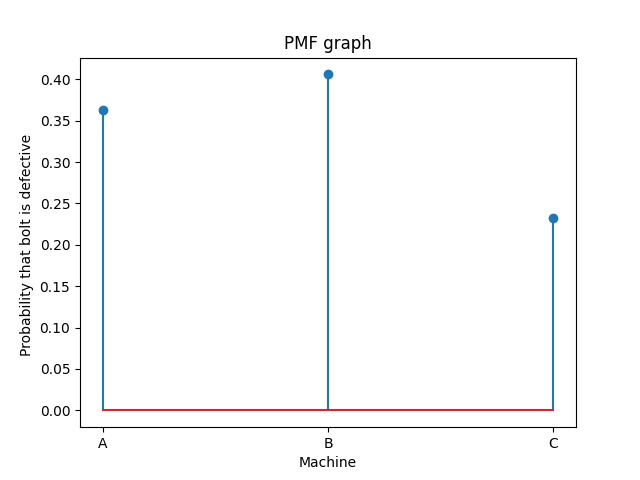
\includegraphics[width=\columnwidth]{Fig-1.png}
\caption{PMF graph}
\label{Fig 1}
\end{figure}
\end{document}